\subsection{Check ECAL linearity response}
\label{linearity}

Here we use MVA BDTG method training on unsaturated electron in MC and apply it to
unsaturated electron in data to check ECAL linearity response for high energy electrons.

The training target defined as:
\begin{eqnarray}
  T & = & \frac{E_{calo}}{E_{24}} \label{equ:ECAL_linearity_target}
\end{eqnarray}
where the $E_{calo}$ is the calorimeter energy of electron and $E_{24}$ is the sum energy of crystals in $5\times5$ matrix without seeded crystal.
The training input variables are listed below:
\begin{itemize}
\item $\frac{E_{left}}{E_{24}}, \frac{E_{right}}{E_{24}}, \frac{E_{top}}{E_{24}}, \frac{E_{bottom}}{E_{24}}$ : energy of the four crystals around the seed normalized to $E_{24}$
\item $\frac{E_{2\times5~ left}}{E_{24}}, \frac{E_{2\times5~ right}}{E_{24}}, \frac{E_{2\times5~top}}{E_{24}}, \frac{E_{2\times5~ bottom}}{E_{24}}$ : energy of the four $2\times5$ crystal dominoes around the seed belonging to the $5\times5$ matrix normalized to $E_{24}$
\item $\frac{E_{preShower}}{E_{24}}$ : energy measured in the PreShower normalized to $E_{24}$ (only for endcap electrons)
\item $\eta$ of the SC
\end{itemize}

The MC samples for training and testing are \texttt{ZToEE\_NNPDF30\_13TeV-powheg\_M\_400\_800 (also 800\_1400)} Moriond sample. The electrons used for training are unsaturated HEEP electrons with calorimeter energy higher than 500 GeV in barrel and 600 GeV in endcap separately. The data used for applying the MVA method are \texttt{DoubleEG\_Run2016B(C,D,E,F,G,H)\\-03Feb2017\_v*\_MINIAOD} datasets ($L \sim 35.9~fb^{-1} $).

\subsubsection{Result}
The result from MC shown in Figure \ref{fig:MC_1} is for electron energy from 500 to 700 GeV in barrel and 600 to 1000 GeV in endcap, the result in Figure \ref{fig:MC_2} is for electron energy more than 700 GeV in barrel and more than 1000 GeV in endcap. Simliarly the result from data shown in Figure \ref{fig:data_1} is for electron energy from 500 to 700 GeV in barrel and 600 to 1000 GeV in endcap, the result in Figure \ref{fig:data_2} is for electron energy more than 700 GeV in barrel and more than 1000 GeV in endcap. In order to reduce the fake electrons in data we require there are two HEEP electrons and at least one in barrel for the data event. So the result from MC in barrel is very good, for endcap the peak has around 1-2\% shift. The result from data is seems fine, the value from MAV has ~1\% lower than the reconstructed energy (calo energy).

\begin{figure}[bh]
  \begin{center}
    \begin{tabular}{cc}
      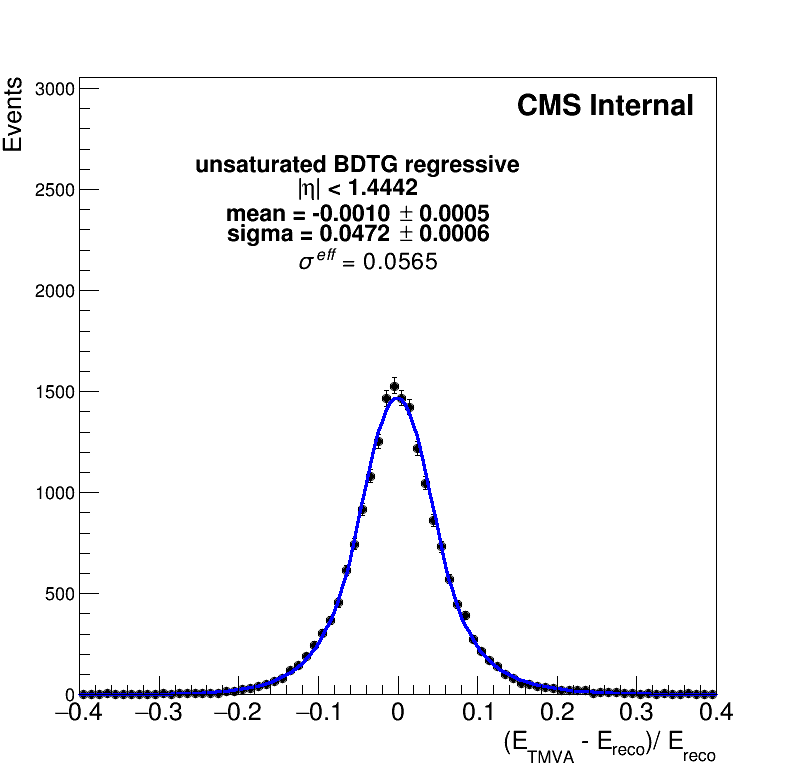
\includegraphics[width=0.45\textwidth]{chapters/Zprime/Saturation/images/ZToEE/ZToEE_B500-700_E600-1000/fit_BDTG_Barrel_Endcap_B_reg_nos.png} &
      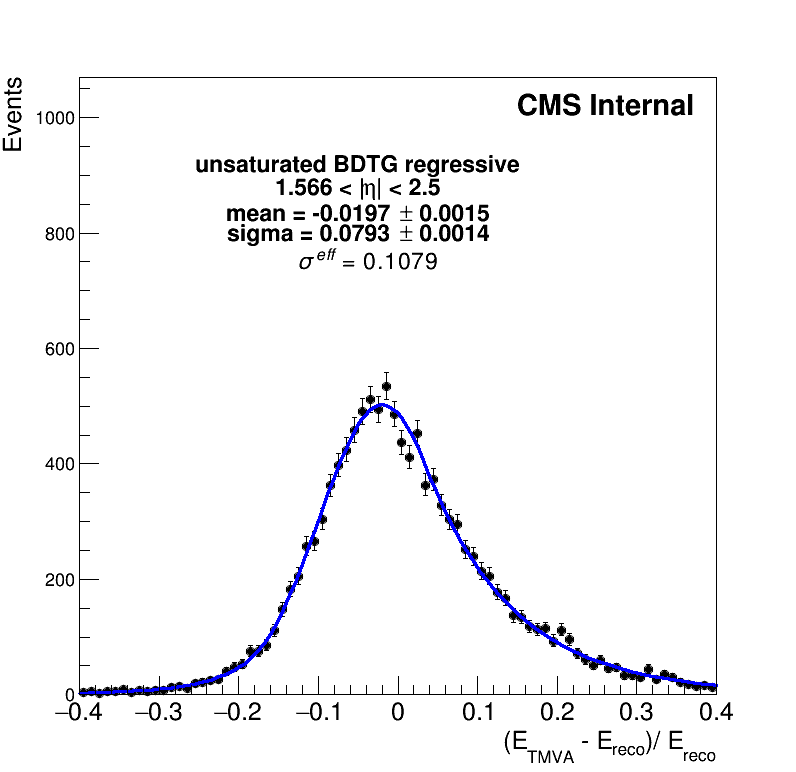
\includegraphics[width=0.45\textwidth]{chapters/Zprime/Saturation/images/ZToEE/ZToEE_B500-700_E600-1000/fit_BDTG_Barrel_Endcap_E_reg_nos.png} \\
    \end{tabular}
    \caption{ The distributions of unsaturated HEEP electrons energy from MVA minus reconstructed energy devide reconstructed energy for barrel for the reconstructed energy between 500 to 700 GeV (left) and for endcap for the reconstructed energy between 600 to 1000 GeV (right) from MC.}
    \label{fig:MC_1}
  \end{center}
\end{figure}


\begin{figure}[bh]
  \begin{center}
    \begin{tabular}{cc}
      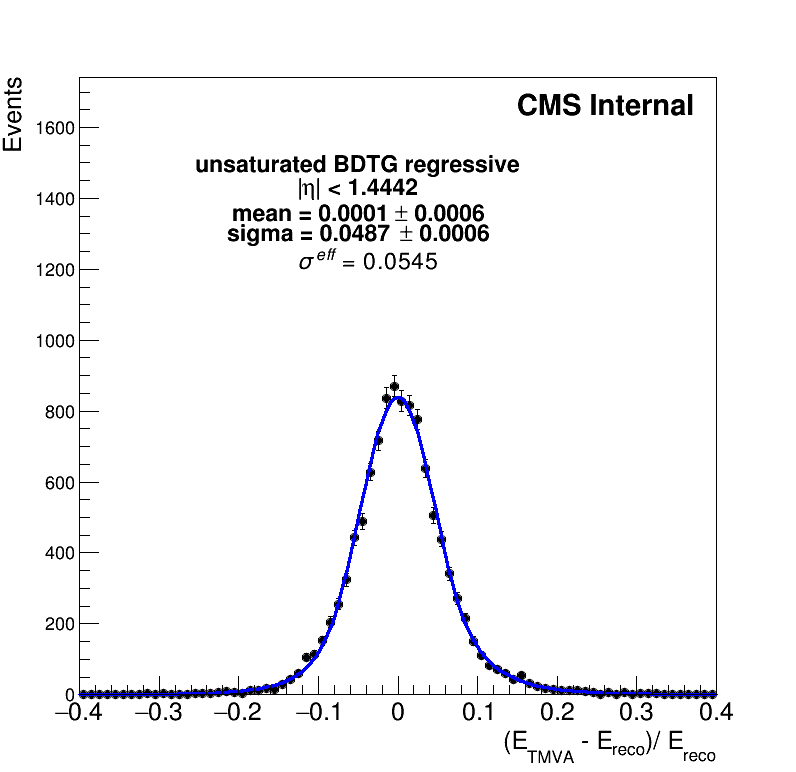
\includegraphics[width=0.45\textwidth]{chapters/Zprime/Saturation/images/ZToEE/ZToEE_B700_E1000/fit_BDTG_Barrel_Endcap_B_reg_nos.png} &
      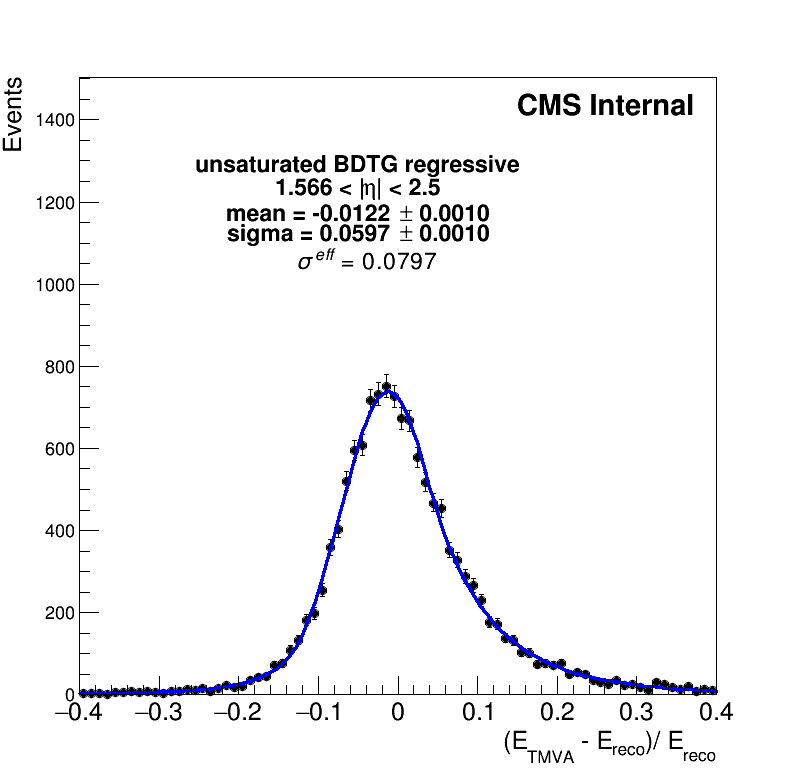
\includegraphics[width=0.45\textwidth]{chapters/Zprime/Saturation/images/ZToEE/ZToEE_B700_E1000/fit_BDTG_Barrel_Endcap_E_reg_nos.png} \\
    \end{tabular}
    \caption{ The distributions of unsaturated HEEP electrons energy from MVA minus reconstructed energy devide reconstructed energy for barrel for the reconstructed energy more than 700 GeV (left) and for endcap for the reconstructed energy more than 1000 GeV (right) from MC.}
    \label{fig:MC_2}
  \end{center}
\end{figure}


\begin{figure}[bh]
  \begin{center}
    \begin{tabular}{cc}
      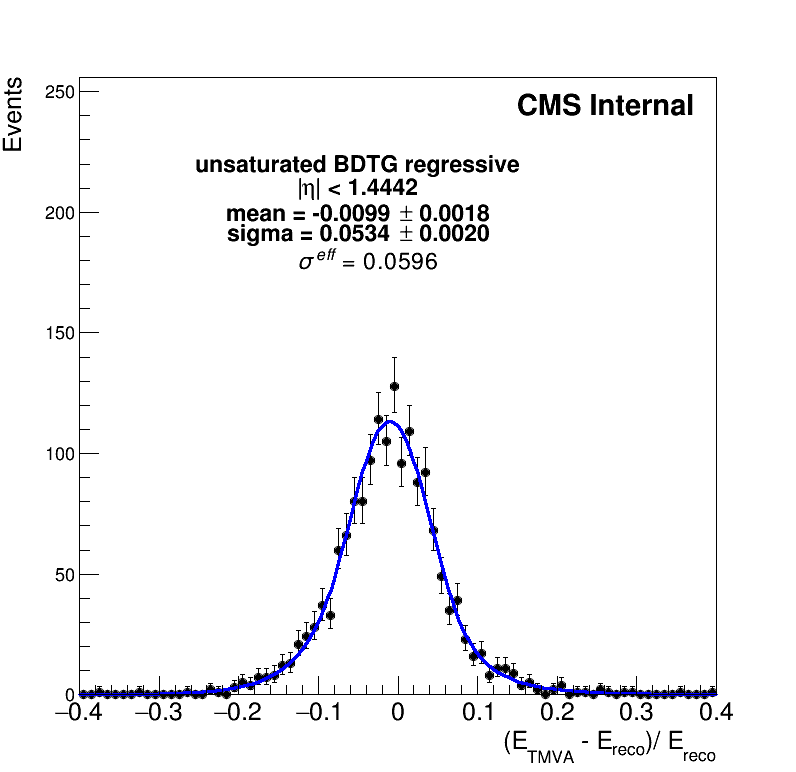
\includegraphics[width=0.45\textwidth]{chapters/Zprime/Saturation/images/ZToEE/data_B500-700_E600-1000/fit_BDTG_Barrel_Endcap_B_reg_nos.png} &
      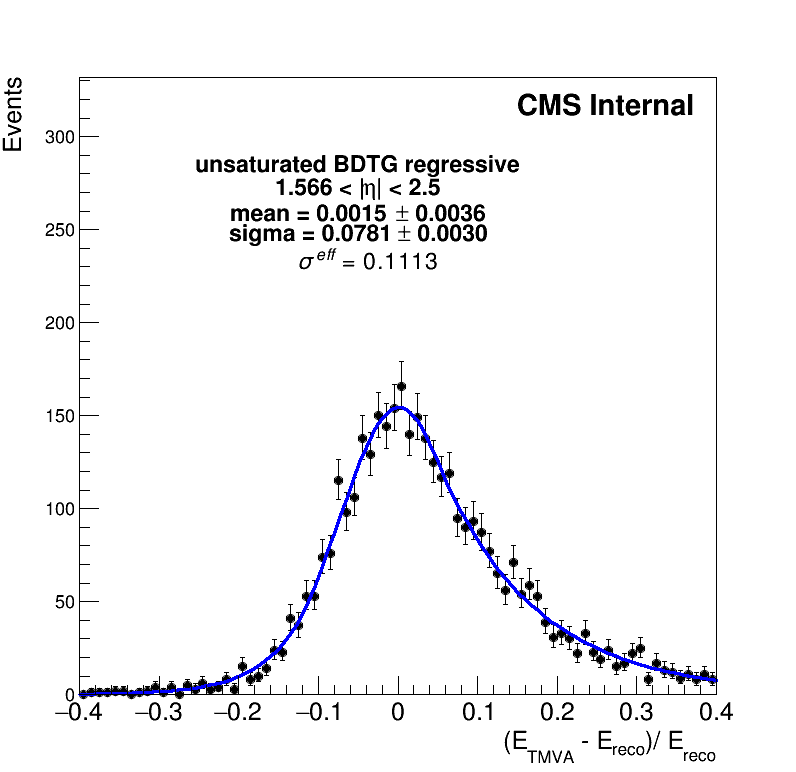
\includegraphics[width=0.45\textwidth]{chapters/Zprime/Saturation/images/ZToEE/data_B500-700_E600-1000/fit_BDTG_Barrel_Endcap_E_reg_nos.png} \\
    \end{tabular}
    \caption{ The distributions of unsaturated HEEP electrons energy from MVA minus reconstructed energy devide reconstructed energy for barrel for the reconstructed energy between 500 to 700 GeV (left) and for endcap for the reconstructed energy between 600 to 1000 GeV (right) from data.}
    \label{fig:data_1}
  \end{center}
\end{figure}


\begin{figure}[bh]
  \begin{center}
    \begin{tabular}{cc}
      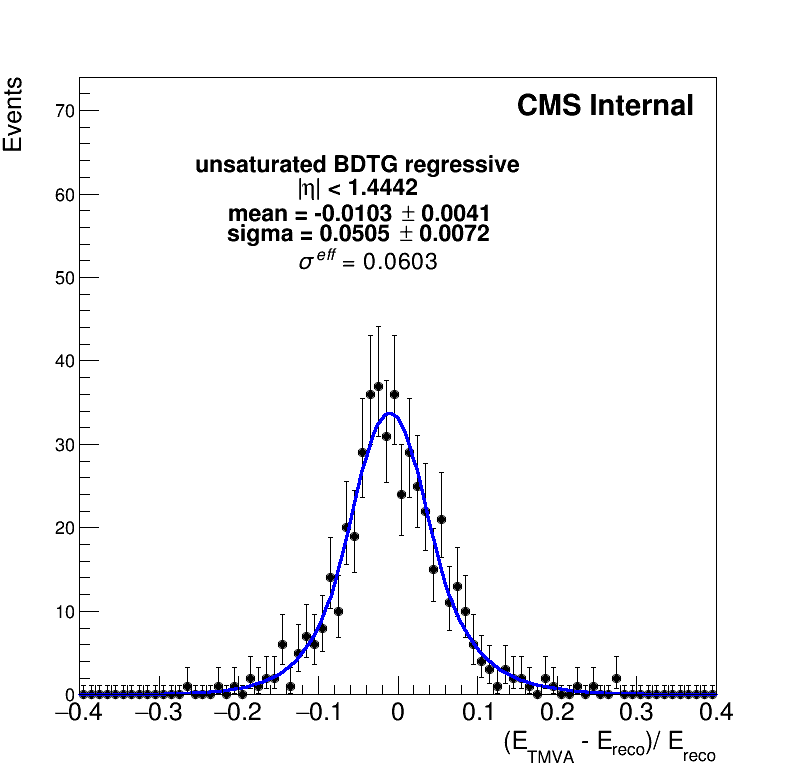
\includegraphics[width=0.45\textwidth]{chapters/Zprime/Saturation/images/ZToEE/data_B700_E1000/fit_BDTG_Barrel_Endcap_B_reg_nos.png} &
      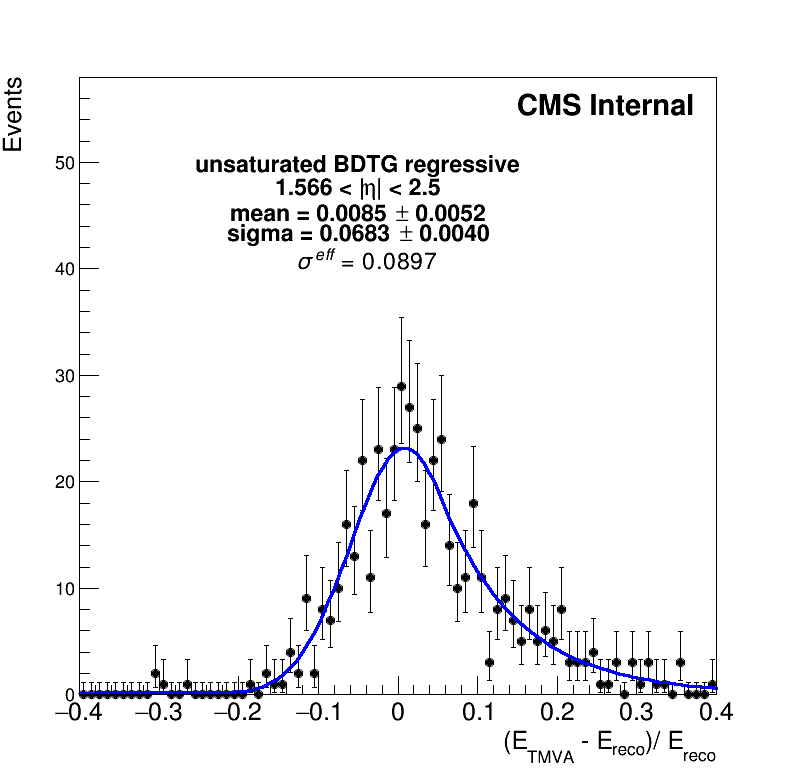
\includegraphics[width=0.45\textwidth]{chapters/Zprime/Saturation/images/ZToEE/data_B700_E1000/fit_BDTG_Barrel_Endcap_E_reg_nos.png} \\
    \end{tabular}
    \caption{ The distributions of unsaturated HEEP electrons energy from MVA minus reconstructed energy devide reconstructed energy for barrel for the reconstructed energy more than 700 GeV (left) and for endcap for the reconstructed energy more than 1000 GeV (right) from data.}
    \label{fig:data_2}
  \end{center}
\end{figure}

